\documentclass[ignorenonframetext,]{beamer}
\setbeamertemplate{caption}[numbered]
\setbeamertemplate{caption label separator}{: }
\setbeamercolor{caption name}{fg=normal text.fg}
\beamertemplatenavigationsymbolsempty
\usepackage{lmodern}
\usepackage{amssymb,amsmath}
\usepackage{ifxetex,ifluatex}
\usepackage{fixltx2e} % provides \textsubscript
\ifnum 0\ifxetex 1\fi\ifluatex 1\fi=0 % if pdftex
  \usepackage[T1]{fontenc}
  \usepackage[utf8]{inputenc}
\else % if luatex or xelatex
  \ifxetex
    \usepackage{mathspec}
  \else
    \usepackage{fontspec}
  \fi
  \defaultfontfeatures{Ligatures=TeX,Scale=MatchLowercase}
\fi
% use upquote if available, for straight quotes in verbatim environments
\IfFileExists{upquote.sty}{\usepackage{upquote}}{}
% use microtype if available
\IfFileExists{microtype.sty}{%
\usepackage{microtype}
\UseMicrotypeSet[protrusion]{basicmath} % disable protrusion for tt fonts
}{}
\newif\ifbibliography
\hypersetup{
            pdftitle={Parallelization and Remote Servers},
            pdfauthor={Abby Bratt, Maria Kuruvilla, and Colin Okasaki},
            pdfborder={0 0 0},
            breaklinks=true}
\urlstyle{same}  % don't use monospace font for urls
\usepackage{color}
\usepackage{fancyvrb}
\newcommand{\VerbBar}{|}
\newcommand{\VERB}{\Verb[commandchars=\\\{\}]}
\DefineVerbatimEnvironment{Highlighting}{Verbatim}{commandchars=\\\{\}}
% Add ',fontsize=\small' for more characters per line
\usepackage{framed}
\definecolor{shadecolor}{RGB}{248,248,248}
\newenvironment{Shaded}{\begin{snugshade}}{\end{snugshade}}
\newcommand{\KeywordTok}[1]{\textcolor[rgb]{0.13,0.29,0.53}{\textbf{#1}}}
\newcommand{\DataTypeTok}[1]{\textcolor[rgb]{0.13,0.29,0.53}{#1}}
\newcommand{\DecValTok}[1]{\textcolor[rgb]{0.00,0.00,0.81}{#1}}
\newcommand{\BaseNTok}[1]{\textcolor[rgb]{0.00,0.00,0.81}{#1}}
\newcommand{\FloatTok}[1]{\textcolor[rgb]{0.00,0.00,0.81}{#1}}
\newcommand{\ConstantTok}[1]{\textcolor[rgb]{0.00,0.00,0.00}{#1}}
\newcommand{\CharTok}[1]{\textcolor[rgb]{0.31,0.60,0.02}{#1}}
\newcommand{\SpecialCharTok}[1]{\textcolor[rgb]{0.00,0.00,0.00}{#1}}
\newcommand{\StringTok}[1]{\textcolor[rgb]{0.31,0.60,0.02}{#1}}
\newcommand{\VerbatimStringTok}[1]{\textcolor[rgb]{0.31,0.60,0.02}{#1}}
\newcommand{\SpecialStringTok}[1]{\textcolor[rgb]{0.31,0.60,0.02}{#1}}
\newcommand{\ImportTok}[1]{#1}
\newcommand{\CommentTok}[1]{\textcolor[rgb]{0.56,0.35,0.01}{\textit{#1}}}
\newcommand{\DocumentationTok}[1]{\textcolor[rgb]{0.56,0.35,0.01}{\textbf{\textit{#1}}}}
\newcommand{\AnnotationTok}[1]{\textcolor[rgb]{0.56,0.35,0.01}{\textbf{\textit{#1}}}}
\newcommand{\CommentVarTok}[1]{\textcolor[rgb]{0.56,0.35,0.01}{\textbf{\textit{#1}}}}
\newcommand{\OtherTok}[1]{\textcolor[rgb]{0.56,0.35,0.01}{#1}}
\newcommand{\FunctionTok}[1]{\textcolor[rgb]{0.00,0.00,0.00}{#1}}
\newcommand{\VariableTok}[1]{\textcolor[rgb]{0.00,0.00,0.00}{#1}}
\newcommand{\ControlFlowTok}[1]{\textcolor[rgb]{0.13,0.29,0.53}{\textbf{#1}}}
\newcommand{\OperatorTok}[1]{\textcolor[rgb]{0.81,0.36,0.00}{\textbf{#1}}}
\newcommand{\BuiltInTok}[1]{#1}
\newcommand{\ExtensionTok}[1]{#1}
\newcommand{\PreprocessorTok}[1]{\textcolor[rgb]{0.56,0.35,0.01}{\textit{#1}}}
\newcommand{\AttributeTok}[1]{\textcolor[rgb]{0.77,0.63,0.00}{#1}}
\newcommand{\RegionMarkerTok}[1]{#1}
\newcommand{\InformationTok}[1]{\textcolor[rgb]{0.56,0.35,0.01}{\textbf{\textit{#1}}}}
\newcommand{\WarningTok}[1]{\textcolor[rgb]{0.56,0.35,0.01}{\textbf{\textit{#1}}}}
\newcommand{\AlertTok}[1]{\textcolor[rgb]{0.94,0.16,0.16}{#1}}
\newcommand{\ErrorTok}[1]{\textcolor[rgb]{0.64,0.00,0.00}{\textbf{#1}}}
\newcommand{\NormalTok}[1]{#1}
\usepackage{graphicx,grffile}
\makeatletter
\def\maxwidth{\ifdim\Gin@nat@width>\linewidth\linewidth\else\Gin@nat@width\fi}
\def\maxheight{\ifdim\Gin@nat@height>\textheight0.8\textheight\else\Gin@nat@height\fi}
\makeatother
% Scale images if necessary, so that they will not overflow the page
% margins by default, and it is still possible to overwrite the defaults
% using explicit options in \includegraphics[width, height, ...]{}
\setkeys{Gin}{width=\maxwidth,height=\maxheight,keepaspectratio}

% Prevent slide breaks in the middle of a paragraph:
\widowpenalties 1 10000
\raggedbottom

\AtBeginPart{
  \let\insertpartnumber\relax
  \let\partname\relax
  \frame{\partpage}
}
\AtBeginSection{
  \ifbibliography
  \else
    \let\insertsectionnumber\relax
    \let\sectionname\relax
    \frame{\sectionpage}
  \fi
}
\AtBeginSubsection{
  \let\insertsubsectionnumber\relax
  \let\subsectionname\relax
  \frame{\subsectionpage}
}

\setlength{\parindent}{0pt}
\setlength{\parskip}{6pt plus 2pt minus 1pt}
\setlength{\emergencystretch}{3em}  % prevent overfull lines
\providecommand{\tightlist}{%
  \setlength{\itemsep}{0pt}\setlength{\parskip}{0pt}}
\setcounter{secnumdepth}{0}
\usepackage{tikz}
\usepackage{pgfplots}
\usepackage{verbatim}
\usepackage{textcomp}
\usetikzlibrary{shapes,arrows}

\title{Parallelization and Remote Servers}
\author{Abby Bratt, Maria Kuruvilla, and Colin Okasaki}
\date{February 5, 2020}

\begin{document}
\frame{\titlepage}

\begin{frame}

\end{frame}

\begin{frame}{Remote Servers: Why Bother?}

\begin{block}{The Basics: How Do Computers Work?}

\begin{itemize}[<+->]
\tightlist
\item
  Computation: CPUs

  \begin{itemize}[<+->]
  \tightlist
  \item
    Each CPU has 1 or more cores
  \item
    Each core can do 1 computation at a time
  \item
    Theoretical top speed = all cores active
  \item
    Reality: cores need to communicate
  \end{itemize}
\item
  Memory: RAM vs.~not-RAM

  \begin{itemize}[<+->]
  \tightlist
  \item
    RAM is volatile, extremely fast, low-volume
  \item
    Hard drive (ex. SSD) is persistent, fairly slow, high-volume
  \end{itemize}
\item
  Sidenote: GPUs and CUDA

  \begin{itemize}[<+->]
  \tightlist
  \item
    Each GPU holds 100s or 1000s of `'CUDA cores''
  \item
    Each CUDA core is very small
  \item
    Very fast for `'embarassingly parallel'' problems
  \end{itemize}
\end{itemize}

\end{block}

\begin{block}{`'Why is my code so slow''}

\begin{itemize}[<+->]
\tightlist
\item
  The most common cases are:

  \begin{itemize}[<+->]
  \tightlist
  \item
    You've run out of RAM
  \item
    Your computer just has too many operations to do
  \end{itemize}
\item
  `'How do I make it faster''

  \begin{itemize}[<+->]
  \tightlist
  \item
    Run it on a bigger computer with more RAM
  \item
    Run it on a bigger computer with more cores
  \end{itemize}
\item
  Solution: use a remote server!
\end{itemize}

\end{block}

\begin{block}{`'Why is my code still so slow''}

Before you use a remote server:

\begin{itemize}[<+->]
\tightlist
\item
  Do some back-of-the-envelope math
\item
  Make sure you don't need an EB of RAM or an EFLOP
\item
  Sidenote: Units

  \begin{itemize}[<+->]
  \tightlist
  \item
    kilo, mega, giga (\(10^9\)), tera (\(10^{12}\)), peta (\(10^{15}\)),
    exa (\(10^{18}\)), zetta, yotta
  \item
    FLOP(S) = floating point operation (per second)
  \item
    newish desktop might have 32 GB RAM, 25 GLOPS speed
  \end{itemize}
\end{itemize}

\end{block}

\begin{block}{(Dis)advantages of parallelization}

\(N\) cores may save you time up to a factor of \(N\), but:

\begin{itemize}[<+->]
\item
  only if you efficiently distribute computation between cores
\item
  only if the programmer-time it takes is relatively small
\item
  Sequential computation: the bane of parallel computation
\item
  Communication: the real bane of parallel computation
\item
  Pre-emptive optimization: the bane of all computation
\end{itemize}

\end{block}

\begin{block}{Example: Conjugate Gradient Descent}

Suppose you wish to calculate \(y = Ax\) but \(A = 10^5 \times 10^5\)

Roughly speaking, \(A\) requites about \(10^{10}\) bytes or 10 GB RAM

Moreover, you need to do \(10^{10}\) multiplications or 10 GFLOPs

Not so bad, but say you want to do this \(10^6\) times (\(\approx\) 6
days)

Luckily \(y_i = \sum A_{ij}x_j\) is independent of all other rows of
\(A\)

Calculating \(y_i\) \(\approx\) 10kB, 10 kFLOPs, GPU takes \(\approx\)
15 minutes

Application: conjugate gradient descent to solve \(Ax = b\)

\end{block}

\begin{block}{Recap: Why use a remote server?}

\begin{itemize}[<+->]
\tightlist
\item
  Lots of CPUs (often a few GPUs) available
\item
  Doesn't slow down your personal computer
\item
  Feel like a pro, brag to your friends
\end{itemize}

\end{block}

\begin{block}{Review}

\begin{itemize}[<+->]
\tightlist
\item
  When should you parallelize?
\item
  When should you definitely not parallelize?
\item
  When should you use a remote server?
\end{itemize}

\end{block}

\begin{block}{Practice}

\begin{itemize}[<+->]
\tightlist
\item
  MCMC
\item
  Bootstrap
\item
  Likelihood evaluation
\item
  Optimization
\end{itemize}

\end{block}

\end{frame}

\begin{frame}{How to Access the QERM/SEFS Servers}

\begin{block}{Some specs}

\begin{itemize}[<+->]
\tightlist
\item
  3 servers

  \begin{itemize}[<+->]
  \tightlist
  \item
    Pilchuk
  \item
    Skykomish
  \item
    Snoqualmie
  \end{itemize}
\item
  24 cores
\item
  256 GB RAM
\item
  1 TB of disk space for temporary storage
\end{itemize}

\end{block}

\begin{block}{Windows}

\begin{itemize}[<+->]
\item
  Remote Desktop Connection
\item
  Enter computer
\item
  Enter your netid and password
\item
  Off campus

  \begin{itemize}[<+->]
  \tightlist
  \item
    download Husky OnNet from
    \href{https://itconnect.uw.edu/connect/uw-networks/about-husky-onnet/use-husky-onnet/terms-conditions/}{UWare}
  \item
    Open BIG-IP Edge Client
  \item
    Connect
  \end{itemize}
\end{itemize}

\end{block}

\begin{block}{Linux}

\begin{itemize}[<+->]
\item
  Launch Remmina (or similar software)
\item
  Make sure it is set to RDP (to connect to Windows based desktop)
\item
  Enter IP addresss
\item
  Enter your netid and password
\item
  Off campus

  \begin{itemize}[<+->]
  \tightlist
  \item
    download Husky OnNet from
    \href{https://itconnect.uw.edu/connect/uw-networks/about-husky-onnet/use-husky-onnet/terms-conditions/}{UWare}
  \item
    Use Firefox to install the f5vpn software on Linux systems
  \end{itemize}
\end{itemize}

\end{block}

\begin{block}{MAC}

\begin{itemize}[<+->]
\item
  Microsoft Remote Desktop Connection
\item
  Enter computer/connection name e.g Pilchuck
\item
  PC name e.g.~pilchuck.sefs.uw.edu
\item
  Enter your netid and password
\item
  Off campus

  \begin{itemize}[<+->]
  \tightlist
  \item
    download Husky OnNet from
    \href{https://itconnect.uw.edu/connect/uw-networks/about-husky-onnet/use-husky-onnet/terms-conditions/}{UWare}
  \item
    Open BIG-IP Edge Client
  \item
    Connect
  \end{itemize}
\end{itemize}

\end{block}

\end{frame}

\begin{frame}[fragile]{A Basic R Program}

\begin{block}{Parallel computing}

\begin{itemize}[<+->]
\tightlist
\item
  Using this
  \href{https://nceas.github.io/oss-lessons/parallel-computing-in-r/parallel-computing-in-r.html}{website}
\item
  Use dataset iris
\item
  Sample randomly from these 100 points
\item
  Run a generalised linear model to see if Species is a function of
  Sepal.length
\item
  Save coefficients of model
\item
  Repeat 10000 times
\end{itemize}

\end{block}

\begin{block}{Parallel Computing}

\begin{Shaded}
\begin{Highlighting}[]
\KeywordTok{head}\NormalTok{(iris,}\DecValTok{10}\NormalTok{)}
\end{Highlighting}
\end{Shaded}

\begin{verbatim}
##    Sepal.Length Sepal.Width Petal.Length Petal.Width Species
## 1           5.1         3.5          1.4         0.2  setosa
## 2           4.9         3.0          1.4         0.2  setosa
## 3           4.7         3.2          1.3         0.2  setosa
## 4           4.6         3.1          1.5         0.2  setosa
## 5           5.0         3.6          1.4         0.2  setosa
## 6           5.4         3.9          1.7         0.4  setosa
## 7           4.6         3.4          1.4         0.3  setosa
## 8           5.0         3.4          1.5         0.2  setosa
## 9           4.4         2.9          1.4         0.2  setosa
## 10          4.9         3.1          1.5         0.1  setosa
\end{verbatim}

\end{block}

\begin{block}{Using doParallel}

\begin{Shaded}
\begin{Highlighting}[]
\KeywordTok{library}\NormalTok{(foreach)}
\KeywordTok{library}\NormalTok{(doParallel)}
\KeywordTok{registerDoParallel}\NormalTok{(numCores)}
\NormalTok{x <-}\StringTok{ }\NormalTok{iris[}\KeywordTok{which}\NormalTok{(iris[,}\DecValTok{5}\NormalTok{] }\OperatorTok{!=}\StringTok{ "setosa"}\NormalTok{), }\KeywordTok{c}\NormalTok{(}\DecValTok{1}\NormalTok{,}\DecValTok{5}\NormalTok{)]}
\NormalTok{trials <-}\StringTok{ }\DecValTok{10000}
\KeywordTok{system.time}\NormalTok{(\{}
\NormalTok{  r <-}\StringTok{ }\KeywordTok{foreach}\NormalTok{(}\KeywordTok{icount}\NormalTok{(trials), }\DataTypeTok{.combine=}\NormalTok{rbind) }\OperatorTok\StringTok{ }\NormalTok{\{}
\NormalTok{    ind <-}\StringTok{ }\KeywordTok{sample}\NormalTok{(}\DecValTok{100}\NormalTok{, }\DecValTok{100}\NormalTok{, }\DataTypeTok{replace=}\OtherTok{TRUE}\NormalTok{)}
\NormalTok{    result1 <-}\StringTok{ }\KeywordTok{glm}\NormalTok{(x[ind,}\DecValTok{2}\NormalTok{]}\OperatorTok{~}\NormalTok{x[ind,}\DecValTok{1}\NormalTok{], }\DataTypeTok{family=}\KeywordTok{binomial}\NormalTok{(logit))}
    \KeywordTok{coefficients}\NormalTok{(result1)}
\NormalTok{  \}}
\NormalTok{\})}
\end{Highlighting}
\end{Shaded}

\begin{verbatim}
##    user  system elapsed 
##    4.55    0.84   12.46
\end{verbatim}

\end{block}

\begin{block}{Without doParallel}

\begin{Shaded}
\begin{Highlighting}[]
\KeywordTok{system.time}\NormalTok{(\{}
\NormalTok{  r <-}\StringTok{ }\KeywordTok{foreach}\NormalTok{(}\KeywordTok{icount}\NormalTok{(trials), }\DataTypeTok{.combine=}\NormalTok{rbind) }\OperatorTok\StringTok{ }\NormalTok{\{}
\NormalTok{    ind <-}\StringTok{ }\KeywordTok{sample}\NormalTok{(}\DecValTok{100}\NormalTok{, }\DecValTok{100}\NormalTok{, }\DataTypeTok{replace=}\OtherTok{TRUE}\NormalTok{)}
\NormalTok{    result1 <-}\StringTok{ }\KeywordTok{glm}\NormalTok{(x[ind,}\DecValTok{2}\NormalTok{]}\OperatorTok{~}\NormalTok{x[ind,}\DecValTok{1}\NormalTok{], }\DataTypeTok{family=}\KeywordTok{binomial}\NormalTok{(logit))}
    \KeywordTok{coefficients}\NormalTok{(result1)}
\NormalTok{  \}}
\NormalTok{\})}
\end{Highlighting}
\end{Shaded}

\begin{verbatim}
##    user  system elapsed 
##   24.64    0.30   25.12
\end{verbatim}

\end{block}

\begin{block}{Using lapply()}

\begin{Shaded}
\begin{Highlighting}[]
\NormalTok{x <-}\StringTok{ }\NormalTok{iris[}\KeywordTok{which}\NormalTok{(iris[,}\DecValTok{5}\NormalTok{] }\OperatorTok{!=}\StringTok{ "setosa"}\NormalTok{), }\KeywordTok{c}\NormalTok{(}\DecValTok{1}\NormalTok{,}\DecValTok{5}\NormalTok{)]}
\NormalTok{trials <-}\StringTok{ }\KeywordTok{seq}\NormalTok{(}\DecValTok{1}\NormalTok{, }\DecValTok{10000}\NormalTok{)}
\NormalTok{boot_fx <-}\StringTok{ }\ControlFlowTok{function}\NormalTok{(trial) \{}
\NormalTok{  ind <-}\StringTok{ }\KeywordTok{sample}\NormalTok{(}\DecValTok{100}\NormalTok{, }\DecValTok{100}\NormalTok{, }\DataTypeTok{replace=}\OtherTok{TRUE}\NormalTok{)}
\NormalTok{  result1 <-}\StringTok{ }\KeywordTok{glm}\NormalTok{(x[ind,}\DecValTok{2}\NormalTok{]}\OperatorTok{~}\NormalTok{x[ind,}\DecValTok{1}\NormalTok{], }\DataTypeTok{family=}\KeywordTok{binomial}\NormalTok{(logit))}
\NormalTok{  r <-}\StringTok{ }\KeywordTok{coefficients}\NormalTok{(result1)}
\NormalTok{  res <-}\StringTok{ }\KeywordTok{rbind}\NormalTok{(}\KeywordTok{data.frame}\NormalTok{(), r)}
\NormalTok{\}}
\KeywordTok{system.time}\NormalTok{(\{}
\NormalTok{  results <-}\StringTok{ }\KeywordTok{lapply}\NormalTok{(trials, boot_fx)}
\NormalTok{\})}
\end{Highlighting}
\end{Shaded}

\begin{verbatim}
##    user  system elapsed 
##   25.53    0.30   25.92
\end{verbatim}

\end{block}

\begin{block}{Using mclapply()}

\begin{Shaded}
\begin{Highlighting}[]
\KeywordTok{library}\NormalTok{(parallel)}
\NormalTok{numCores <-}\StringTok{ }\KeywordTok{detectCores}\NormalTok{()}
\NormalTok{numCores}
\end{Highlighting}
\end{Shaded}

\begin{verbatim}
## [1] 4
\end{verbatim}

\end{block}

\begin{block}{Using mclapply()}

\begin{Shaded}
\begin{Highlighting}[]
\NormalTok{x <-}\StringTok{ }\NormalTok{iris[}\KeywordTok{which}\NormalTok{(iris[,}\DecValTok{5}\NormalTok{] }\OperatorTok{!=}\StringTok{ "setosa"}\NormalTok{), }\KeywordTok{c}\NormalTok{(}\DecValTok{1}\NormalTok{,}\DecValTok{5}\NormalTok{)]}
\NormalTok{trials <-}\StringTok{ }\KeywordTok{seq}\NormalTok{(}\DecValTok{1}\NormalTok{, }\DecValTok{10000}\NormalTok{)}
\NormalTok{boot_fx <-}\StringTok{ }\ControlFlowTok{function}\NormalTok{(trial) \{}
\NormalTok{  ind <-}\StringTok{ }\KeywordTok{sample}\NormalTok{(}\DecValTok{100}\NormalTok{, }\DecValTok{100}\NormalTok{, }\DataTypeTok{replace=}\OtherTok{TRUE}\NormalTok{)}
\NormalTok{  result1 <-}\StringTok{ }\KeywordTok{glm}\NormalTok{(x[ind,}\DecValTok{2}\NormalTok{]}\OperatorTok{~}\NormalTok{x[ind,}\DecValTok{1}\NormalTok{], }\DataTypeTok{family=}\KeywordTok{binomial}\NormalTok{(logit))}
\NormalTok{  r <-}\StringTok{ }\KeywordTok{coefficients}\NormalTok{(result1)}
\NormalTok{  res <-}\StringTok{ }\KeywordTok{rbind}\NormalTok{(}\KeywordTok{data.frame}\NormalTok{(), r)}
\NormalTok{\}}
\KeywordTok{system.time}\NormalTok{(\{}
\NormalTok{  results <-}\StringTok{ }\KeywordTok{mclapply}\NormalTok{(trials, boot_fx, }\DataTypeTok{mc.cores =} \DecValTok{1}\NormalTok{)}
\NormalTok{\})}
\end{Highlighting}
\end{Shaded}

\begin{verbatim}
##    user  system elapsed 
##   25.38    0.19   25.61
\end{verbatim}

\end{block}

\end{frame}

\begin{frame}[fragile]{How to Access Hyak}

\begin{block}{What is hyak?}

Hyak is a word in Chinook Jargon, meaning ``fast.'' Chinook Jargon is
the trade language of the Pacific Northwest, incorporating terms from
Chinook and Chehalis and other local languages, as well as French and
English. We've chosen words from Chinook Jargon for the names of systems
in the UW research cyber infrastructure to emphasize their role in
supporting the broad range of UW research users and our ties to our
place between the mountains and Salish Sea.

--UW IT Connect

\end{block}

\begin{block}{What is hyak?}

Hyak is part of an integrated, scalable, scientific super-computing
infrastructure operated by UW-IT. It includes the lolo tapearchive
system, a high-performance research network, \textbf{the Hyak compute
infrastructure (the HPC clusters)}, and any scientific support services
on making this useful in your research workflows.

--UW IT Connect

\end{block}

\begin{block}{How does hyak work?}

Within hyak, \textbf{mox} is a supercomputing \textbf{cluster}.

A \textbf{cluster} is a set of connected computers, \textbf{nodes}, that
work together in a single system.

In general, \textbf{clusters} are faster and more capable than a single
computer or even several disconnected computers.

--UW Research Computing Club

\end{block}

\begin{block}{How does hyak work?}

On mox, labs or groups can buy groups of nodes called
\textbf{partitions}. The Research Computing Club applied for a big grant
from the Student Technology Fee fund (that we all pay into every
quarter!) to purchase nodes accessible to all students.

\end{block}

\begin{block}{How does hyak work?}

\begin{itemize}[<+->]
\item
  In general, the compute nodes have the following specs:

  \begin{itemize}[<+->]
  \item
    28 cores
  \item
    128 GB RAM
  \end{itemize}
\item
  The STF partition is currently 92 regular nodes, plus some interactive
  and GPU nodes.
\item
  That's a lot
\end{itemize}

\end{block}

\begin{block}{How does hyak work?}

\begin{itemize}[<+->]
\tightlist
\item
  Login nodes (mox1, mox2)

  \begin{itemize}[<+->]
  \tightlist
  \item
    Have internet
  \item
    Use these to upload/download files and submit jobs
  \item
    They are slow so \textbf{don't} do heavy processing
  \end{itemize}
\end{itemize}

\end{block}

\begin{block}{How does hyak work?}

\begin{itemize}[<+->]
\tightlist
\item
  Login nodes (mox1, mox2)

  \begin{itemize}[<+->]
  \tightlist
  \item
    Have internet
  \item
    Use these to upload/download files and submit jobs
  \item
    They are slow so \textbf{don't} do heavy processing
  \end{itemize}
\item
  Build nodes (n\#\#\#\#\#)

  \begin{itemize}[<+->]
  \tightlist
  \item
    Have internet
  \item
    Don't get to take a whole node (so also kinda slow)
  \item
    Just for compiling software
  \end{itemize}
\item
  Compute nodes (n\#\#\#\#\#)

  \begin{itemize}[<+->]
  \tightlist
  \item
    No internet
  \item
    Where your jobs run
  \end{itemize}
\end{itemize}

Visually, this looks like:

\begin{figure}
\centering
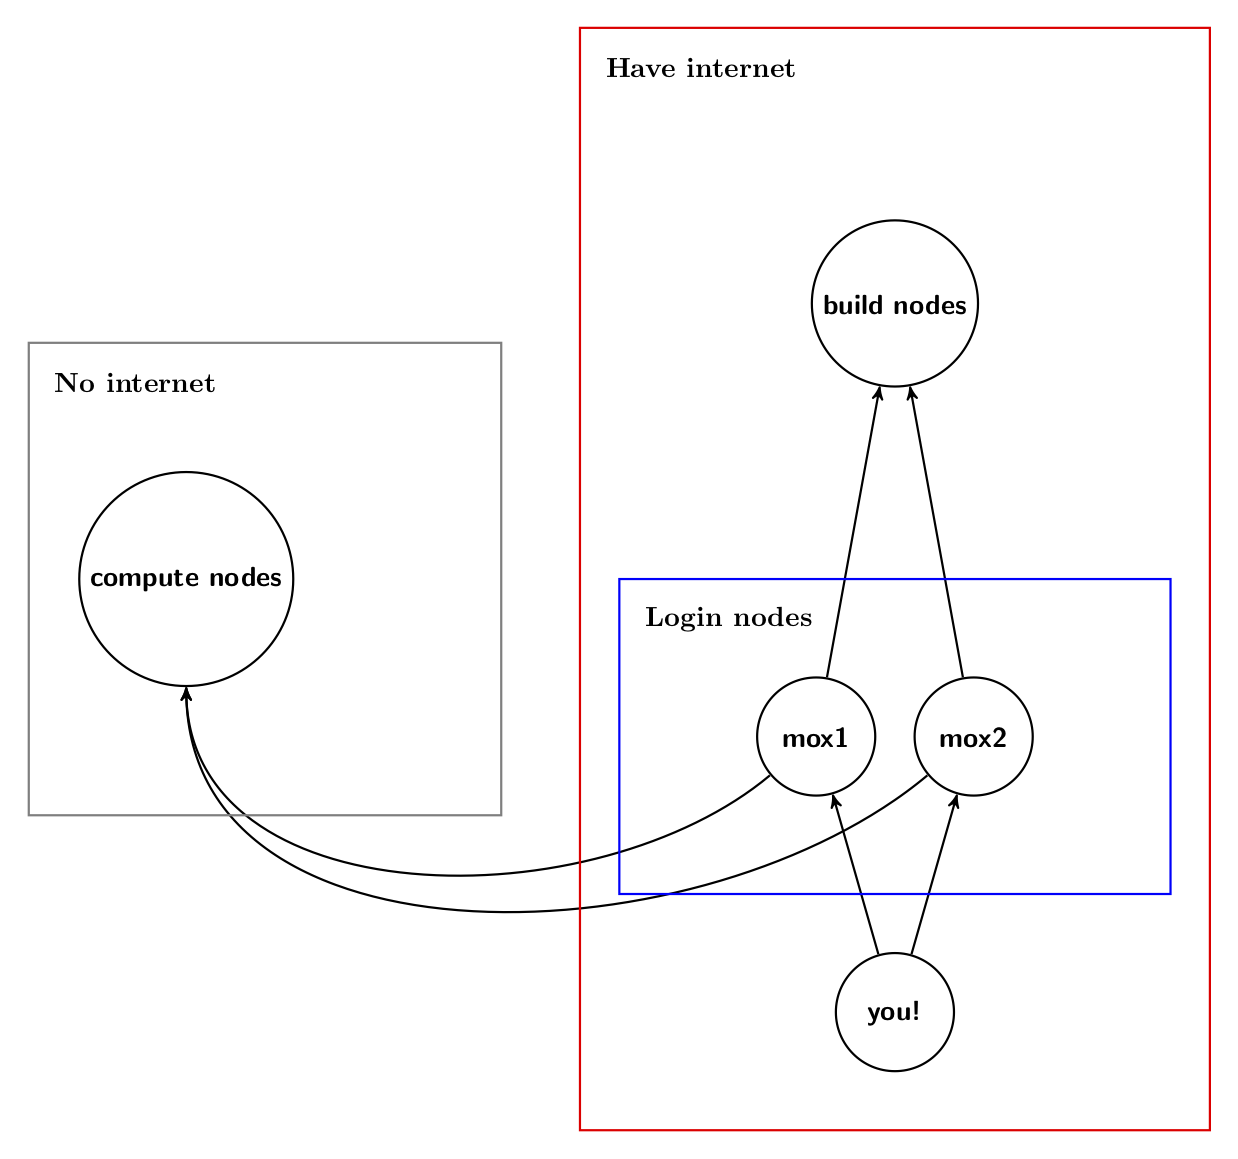
\includegraphics[width=5.20833in]{images/Hyak_architecture.png}
\caption{}
\end{figure}

\end{block}

\begin{block}{How do I log in?}

All nodes share the same file system.

Open a terminal window. Type

\begin{verbatim}
ssh UWNETID@mox.hyak.uw.edu
\end{verbatim}

Follow two-factor authentication instructions.

You're in!

\end{block}

\begin{block}{It should look like this\ldots{}}

\begin{figure}
\centering

\includegraphics[width=6.25000in]{images/Hyak_successful_login.png}
\caption{}
\end{figure}

\end{block}

\begin{block}{Exercise}

Log in!

\end{block}

\begin{block}{Important locations}

\begin{itemize}[<+->]
\tightlist
\item
  /gscratch/stf

  \begin{itemize}[<+->]
  \tightlist
  \item
    Main work location for stf users
  \item
    Any files untouched for \textgreater{}30 days will be scrubbed!!
  \end{itemize}
\item
  /usr/lusers/

  \begin{itemize}[<+->]
  \tightlist
  \item
    Home directory
  \item
    Only 10 GB of storage per user
  \end{itemize}
\item
  /tmp

  \begin{itemize}[<+->]
  \tightlist
  \item
    Node local storage
  \end{itemize}
\end{itemize}

\end{block}

\begin{block}{How do I upload files?}

From GitHub:

\begin{verbatim}
git clone git@github.com:GITHUB-USERNAME/REPO-NAME
\end{verbatim}

From your computer:

\begin{verbatim}
scp filename UWNETID@mox.hyak.uw.edu:/path/to/destination/directory
\end{verbatim}

\end{block}

\begin{block}{Exercise}

Clone the git repo for this class to \textbf{your} scratch directory

\end{block}

\begin{block}{Exercise}

Clone the git repo for this class to \textbf{your} scratch directory

\textbf{Hint:}

From login

\begin{verbatim}
cd /gscratch/stf
mkdir ./UWNETID
cd ./UWNETID
git clone git@github.com:GITHUB-USERNAME/REPO-NAME
cd REPO-NAME
\end{verbatim}

\textbf{Bonus:}

Why use the scratch directory?

\end{block}

\begin{block}{What is a batch script?}

\begin{itemize}[<+->]
\item
  Place to:

  \begin{itemize}[<+->]
  \item
    Define all the options for a job you submit to the queue
  \item
    Set up environment (e.g.~load modules)
  \item
    Run!
  \end{itemize}
\item
  Syntax:

  \begin{itemize}[<+->]
  \item
    Comment using \#\#
  \item
    Set option using \#SBATCH
  \end{itemize}
\end{itemize}

\end{block}

\begin{block}{How do I write a batch script?}

Short answer: don't.

Modify a template! Here's one:

\begin{verbatim}
vim Hyak_simple_batch.sh
\end{verbatim}

Or open this file in your favorite text editor

\end{block}

\begin{block}{It should look like this\ldots{}}

\begin{figure}
\centering
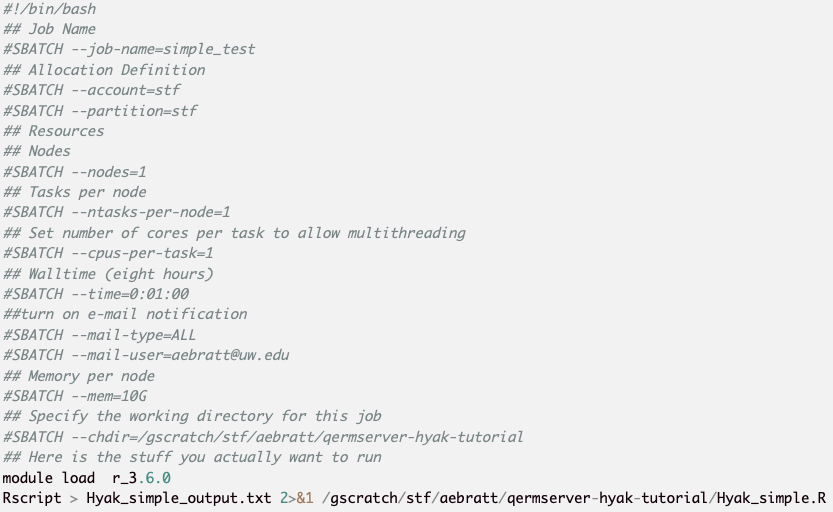
\includegraphics[width=6.25000in]{images/Hyak_simple_batch.png}
\caption{}
\end{figure}

\end{block}

\begin{block}{Exercise}

Submit a job to the queue!

\end{block}

\begin{block}{Exercise}

Submit a job to the queue!

\textbf{Hint:}

First, open vim or another text editor and replace UWNETID in
Hyak\_simple\_batch.sh

\begin{verbatim}
cd /gscratch/stf/UWNETID/qermserver-hyak-tutorial
sbatch -p stf -A stf Hyak_simple_batch.sh
\end{verbatim}

\end{block}

\begin{block}{Wait, what if I need some special library or software?}

You can do that! For R libraries,

\begin{verbatim}
mkdir /gscratch/stf/UWNETID/rpackages
srun -p build --time=2:00:00 --mem=10G --pty /bin/bash
\end{verbatim}

We just created a directory for storing installed packages and got a
session on an \textbf{interactive} build node.

\end{block}

\begin{block}{Wait, what if I need some special library or software?}

Open the command line

\begin{verbatim}
module load r_3.6.0
module list
R
install.packages("PACKAGENAME", lib="/gscratch/stf/UWNETID/rpackages")
\end{verbatim}

Choose a mirror somewhere on the west coast and press enter.

\end{block}

\begin{block}{Exercise}

Submit a more complicated job to the queue!

\textbf{Hint:}

First, open vim or another text editor and replace UWNETID in
Hyak\_complicated.R and Hyak\_complicated\_batch.sh

\begin{verbatim}
exit
cd /gscratch/stf/UWNETID/qermserver-hyak-tutorial
sbatch -p stf -A stf Hyak_complicated_batch.sh
\end{verbatim}

\end{block}

\begin{block}{When will my jobs run?}

See the whole stf partition queue this way:

\begin{verbatim}
squeue -p stf
\end{verbatim}

See just your jobs this way:

\begin{verbatim}
squeue -p stf -u UWNETID
\end{verbatim}

You can also try:

\begin{verbatim}
sstat -j JOBID-RUNNING
sacct -j JOBID-COMPLETED
\end{verbatim}

\end{block}

\begin{block}{Oops, I made a mistake!}

Cancel jobs with

\begin{verbatim}
scancel JOBID#
\end{verbatim}

\end{block}

\begin{block}{My job finished! How do I download my results?}

From Hyak to GitHub:

\begin{verbatim}
git add filename
git commit -m "informative commit message"
git push
\end{verbatim}

From Hyak to your computer:

\begin{verbatim}
scp UWNETID@mox.hyak.uw.edu:/path/to/file .
\end{verbatim}

\end{block}

\begin{block}{How can I get higher priority?}

You can check the priority of queued jobs with

\begin{verbatim}
sprio -p stf
\end{verbatim}

How to interpret?

It may look something like

\begin{figure}
\centering
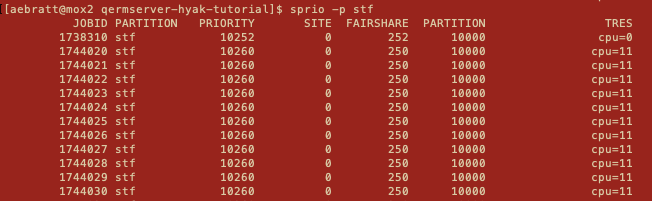
\includegraphics[width=6.25000in]{images/Hyak_priority.png}
\caption{}
\end{figure}

\end{block}

\begin{block}{How can I get higher priority?}

\begin{itemize}[<+->]
\item
  \textbf{TRES}: Trackable RESources (TRES) are things like cpu, memory,
  nodes. The more a given TRES Type is requested/allocated on a job, the
  greater the job priority will be for that job. Mox cares about cpu
  (i.e.~high CPU gets high priority)
\item
  \textbf{Fair-share}: The fair-share component to a job's priority
  influences the order in which a user's queued jobs are scheduled to
  run based on the portion of the computing resources they have been
  allocated and the resources their jobs have already consumed. High
  priority to under-serviced accounts.
\item
  Do not specify a walltime way longer than your job needs.
\item
  Specify your memory! For 128G nodes use --mem=120G or less. The
  operating system requires some.
\end{itemize}

\end{block}

\begin{block}{What else can I do?}

\begin{itemize}[<+->]
\item
  Use the checkpoint queue - run your code on other groups' unused
  resources
\item
  Install and build new software
\end{itemize}

\end{block}

\begin{block}{Where do I get help?}

If you have trouble or you want to do more advanced stuff, check out

\begin{verbatim}
man SLURMCOMMAND
\end{verbatim}

If all else fails, try

\begin{itemize}[<+->]
\item
  Research Computing Club
\item
  eScience Institute
\item
  UW IT
\end{itemize}

\end{block}

\end{frame}

\end{document}
